\documentclass[t,xcolor={svgnames,table}]{beamer}

\usepackage[utf8]{inputenc} % allow utf-8 input
\usepackage[T1]{fontenc}    % use 8-bit T1 fonts
\usepackage[svgnames,table]{xcolor}
\usepackage[none]{hyphenat}
\usepackage{graphicx}
\usepackage{array}
\usepackage[font=small,labelfont=bf]{caption}
\usepackage{amsfonts, amsmath, amsthm, amssymb}
\usepackage{adjustbox}
\usepackage[absolute,overlay]{textpos}
\usepackage{multirow}
\usepackage{cuted}
\usepackage[inline]{enumitem}
\usepackage{url}
\usepackage{tikz,pgfplots,pgfplotstable}
\usepackage[most]{tcolorbox}
\usepackage[charter]{mathdesign}
\usepackage{subcaption}
\usepackage{multirow}
\usetikzlibrary{arrows.meta}
\captionsetup{labelformat=empty}
\graphicspath{{figures/}}

\begin{document}

\begin{frame}
\frametitle{Syntactic Interchangeability in Word Embedding Models}
  \textbf{Daniel Hershcovich} \& \textbf{Assaf Toledo} \& \\
  \textbf{Alon Halfon} \& \textbf{Noam Slonim}
  \hfill
  \textbf{IBM Research}
  \vfill
  
  \begin{adjustbox}{margin=5,frame,minipage=\textwidth,center,color=purple}
    Word embeddings trained with larger context windows --- \\
    capture semantic similarity better \textit{but} are less sensitive to POS
  \end{adjustbox}
  \vfill
  
  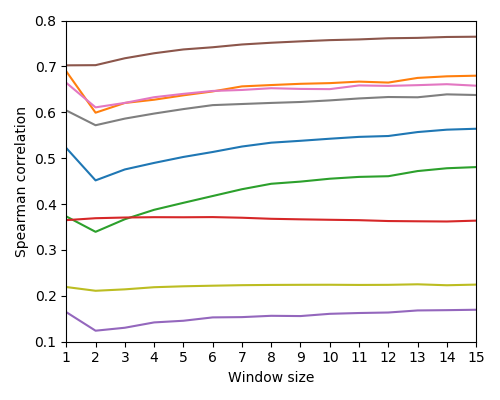
\includegraphics[width=.48\textwidth,trim=17mm 13mm 0 0,clip]{similarities_fasttext_enwiki-20170501-clean_cbow-300d-min500_eval.png}
  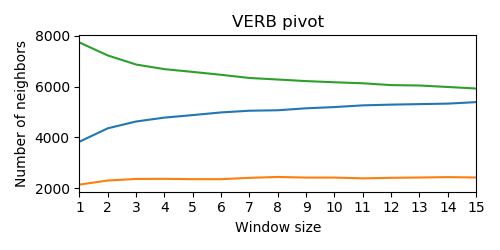
\includegraphics[width=.5\textwidth,trim=2cm 14mm 0 7.5mm,clip,height=33mm]{VERB_nn_100_fasttext_enwiki-20170501-clean_cbow-300d-min500_pos.png}
  Similarity benchmark scores \hfill Nearest neighbor interchangeability

\end{frame}

\end{document}
